% This is samplepaper.tex, a sample chapter demonstrating the
% LLNCS macro package for Springer Computer Science proceedings;
% Version 2.20 of 2017/10/04
%
\documentclass[runningheads]{llncs}

%
\usepackage{graphicx}

\usepackage{todonotes}

% \usepackage[sorting=none]{biblatex}
% \bibliographystyle{ieeetr}
% \bibliography{src/citations.bib}


% Used for displaying a sample figure. If possible, figure files should
% be included in EPS format.
%
% If you use the hyperref package, please uncomment the following line
% to display URLs in blue roman font according to Springer's eBook style:
% \renewcommand\UrlFont{\color{blue}\rmfamily}

\usepackage{float}
\usepackage{bera}% optional: just to have a nice mono-spaced font
\usepackage{listings}
\usepackage{xcolor}

\colorlet{punct}{red!60!black}
\definecolor{background}{HTML}{FAFAFA}
\definecolor{delim}{RGB}{20,105,176}
\colorlet{numb}{magenta!60!black}

\lstdefinelanguage{json}{
    basicstyle=\normalfont\ttfamily,
    numbers=none,
    numberstyle=\scriptsize,
    stepnumber=1,
    numbersep=8pt,
    showstringspaces=false,
    breaklines=false,
    frame=none,% frame=lines,
    backgroundcolor=\color{background},
    literate=
     *{0}{{{\color{numb}0}}}{1}
      {1}{{{\color{numb}1}}}{1}
      {2}{{{\color{numb}2}}}{1}
      {3}{{{\color{numb}3}}}{1}
      {4}{{{\color{numb}4}}}{1}
      {5}{{{\color{numb}5}}}{1}
      {6}{{{\color{numb}6}}}{1}
      {7}{{{\color{numb}7}}}{1}
      {8}{{{\color{numb}8}}}{1}
      {9}{{{\color{numb}9}}}{1}
      {:}{{{\color{punct}{:}}}}{1}
      {,}{{{\color{punct}{,}}}}{1}
      {\{}{{{\color{delim}{\{}}}}{1}
      {\}}{{{\color{delim}{\}}}}}{1}
      {[}{{{\color{delim}{[}}}}{1}
      {]}{{{\color{delim}{]}}}}{1},
}


%%%%%%%%%%%%%%%%%%%%%%%%%%%%%%%%%%%%%%%%%%%
%%%%%%%%%%% Write Nothing Twice %%%%%%%%%%%
%%%%%%%%%%%%%%%%%%%%%%%%%%%%%%%%%%%%%%%%%%%
\newcommand{\serverlocation}{Germany}
\newcommand{\abbrv}[1]{\textit{(#1)}}

\begin{document}
%
\title{
    Analysis of attack patterns on honeypot server
    % \thanks{Supported by organization x.}
}
%
%\titlerunning{Abbreviated paper title}
% If the paper title is too long for the running head, you can set
% an abbreviated paper title here
%
\author{Benedikt H. Thordarson }%\and
% Second Author\inst{2,3}\orcidID{1111-2222-3333-4444} \and
% Third Author\inst{3}\orcidID{2222--3333-4444-5555}}
%
% \authorrunning{F. Author et al.}
% First names are abbreviated in the running head.
% If there are more than two authors, 'et al.' is used.
%
\institute{Reykjavik University, Menntavegur 1, Reykjavik, Iceland } % \and
% Springer Heidelberg, Tiergartenstr. 17, 69121 Heidelberg, Germany
% \email{lncs@springer.com}\\
% \url{http://www.springer.com/gp/computer-science/lncs} \and
% ABC Institute, Rupert-Karls-University Heidelberg, Heidelberg, Germany\\
% \email{\{abc,lncs\}@uni-heidelberg.de}}
%
\maketitle              % typeset the header of the contribution
%


\begin{abstract}
    In this paper, I will present the results from
    recording and comparing the attack patterns 
    experienced by honeypot servers in different 
    geographical regions. 

\keywords{Security  \and Honeypot.}
% ToDo: find more keywords

\end{abstract}
%
%
%
\section{Introduction}
\label{sec:introduction}

    If you have a device connected to the
    internet, it is almost certain that some person,
    or an infected machine has probed it, and possibly
    attempted to break into your device. 


    A 2017 study \cite{Britton_Liu}
    used HoneyPot servers to record malicious
    incoming traffic. Over a 24 hour period they 
    experienced 300,103 attempted attacks, or 
    about 3.4 attacks per second on average.
    These attacks were recorded on devices that
    had no associated domain name, and was in no
    way transmitting any data into the internet
    before being probed.

    
    Currently, there is a rising trend of introducing
    the internet-of-things \textit{(IoT)} devices to 
    home, and industrial environments. The number of 
    IoT devices is currently estimated to be 26.66 
    billion, and by 2025, the count is projected to 
    reach 75.44 billion. \cite{statista}

    
    Most of these IoT devices are similar to the honeypots
    described by Britton et al\cite{Britton_Liu}, in that 
    they are usually small devices, not associated with 
    a hostname, and due to the specialized nature, their 
    communication with the wider internet is limited.


    The overproliferation of these IoT devices has given 
    massive fodder to Botnets such as Mirai, which in 2016
    launched a 620 Gbps attack on KrebsOnSecurity.com
    \cite{Brian_Krebs_2016}.

    
    If
\section{Related Work}
\label{sec:relatedWork}


An 2004 analysis by F. Rainal et al. \cite{1324605}
on network traffic, found that from the first 
seconds of being connected to the internet, the 
honeypot is subject to scans. The amount of time 
ago the experiment was conducted makes it difficult
to compare to, since in the 15 years passed since the
publication, the landscape of the internet has changed 
considerably. 
The authors  make no attempt to discern a pattern
in the scans, or attacks made on the server. They also
point out that a sufficiently skilled intruder, may 
realize that he is in a honeypot, and exit so that 
his intentions are not revealed.


In a 2013, I. Koniaris, G. Papadimitriou, and 
P. Nicopolitidis published a paper outlining
their analysis of four months of honeypot 
activity \cite{6624967}.
 While their project was in many ways
similar to this one, their focus was on 
username and password combinations rather than
exploring the correlation of time of day and 
rate of attacks. 


A similar paper from 2011, describes a statistical 
analysis on honeypot activity 
\cite{Song:2011:SAH:1978672.1978676}. 
The authors however do not attempt to discern a 
pattern from the attacks. In addition, the 8 years
since the paper's publication mean that the 
nature of the internet has changed significantly. 


The use of honeypots has led to anti-honeypot technology.
Krawetz \cite{1264861} 
notes in his 2004 article that spammers are re-active,
not proactive, changing their tools only when they 
become ineffective. The same can be claimed with honeypot
technology, as when a detection strategy is discovered
it will be made ineffective. There indeed is certainly 
evidence of an ongoing arms race, as shown by activity
of attackers on the honeypot, when after logging in, the
attackers check automatically if the attacker is inside a 
busybox.


To understand where the traffic to the server originates from
it is important to acknowledge the existence of large-scale 
botnets\cite{AbuRajab:2006:MAU:1177080.1177086}, automatic
probes, and current scanning technology \cite{6657498}.


\section{Methods}
  \label{sec:methods}
  

  To gather the data I need, I will use the Modern Honey 
  Network\textit{(MHN)} to manage 
  and deploy the HoneyPot server. MHN will collect data about
  the attacks as they take place, and store it in a database.

  For hosting, I choose DigitalOcean, for the ability to
  cheaply run my server in a foreign country.
  The attack patterns can 


  For this study, I will be focusing on SSH brute force attacks.
  To collect data I will use the Cowrie\cite{Cowrie}
  honeypot. An medium interaction SSH and Telnet honeypot
  designed to log brute force attacks and the shell 
  interaction performed by the attacker. A sample session 
  log can be seen in listing \ref{lst:data}

  
  This data includes a timestamp, IP-address,
  target-protocol,
  the credentials that were used to log into the 
  server, and even the commands that were run when
  the attacker thought he had gained access.

  
  By using publicly available databases like
  MaxMind's GeoIP2 City and Country CSV Databases
  \cite{maxminds}, the IP addresses can be translated
  into countries of origins.
  This enables us to break down the attacks by country 
  % (see figure \ref{fig:country_breakdown})

  It is important to note, that while each attack is 
  timestamped, the timestamp is in the timezone of the 
  attacked server, not the attacker. To more accurately
  analyse the rate of launched attacks over day, the
  geo-location can also be used to adjust the timestamp
  to represent the time of which the attack was launched.

  
  The manipulation of the in all ways as described above
  can be achieved by using python, and the existing Pandas
  \cite{pandas} library, which makes the handling and
  aggregation of data easy, and also allows for plotting
  the data.


  
\begin{figure}[H]
\begin{lstlisting}[language=json, 
    caption={Sample attack data gathered from the London HoneyPot. (ID fields omitted for brevity.)},
    captionpos=b, label={lst:data}]

    { 
        "payload": {
            "commands": [], 
            "credentials": [], 
            "endTime": "2019-02-26T14:43:38.820991Z", 
            "hashes": [], 
            "hostIP": "68.183.213.102", 
            "hostPort": 22, 
            "loggedin": [
            "root", 
            "admin"
            ], 
            "peerIP": "5.188.86.174", 
            "peerPort": 52790, 
            "protocol": "ssh", 
            "startTime": "2019-02-26T14:40:38.669266Z", 
            "ttylog": null, 
            "unknownCommands": [], 
            "urls": [], 
            "version": "'SSH-2.0-OpenSSH_7.3'"
        }, 
        "timestamp": "2019-02-26T14:43:38.840000"
    }, 

    \end{lstlisting}
\end{figure}
\section{Results}
\label{sec:results}

    The honeypot records both time stamps, and 
    interaction logs. Analysis of each will be handled separately 
    in subsections \ref{sec:time_analysis} and 
    \ref{sec:session_analysis}. 

    Then in section \ref{sec:irish_analysis} I take 
    a brief look at the origins of attacks.

\subsection{Statistical analysis of attack data}
\label{sec:time_analysis}

    The honeypot has been active since 12. of January
    2019, and until the 19. of March has logged 
    812013 individual SSH attacks. 


    The rate of attacks has been relatively constant over
    time (see figure \ref{fig:attacks_over_time}), with 
    the notable exception of the 12. of January and of 25. 
    January. The low amount of attacks on 12. of January is due 
    to how late I set the server up. 
    The dip in attack rate on the 25 is as of yet 
    unexplained.


    \begin{figure}[H]
        \centering
        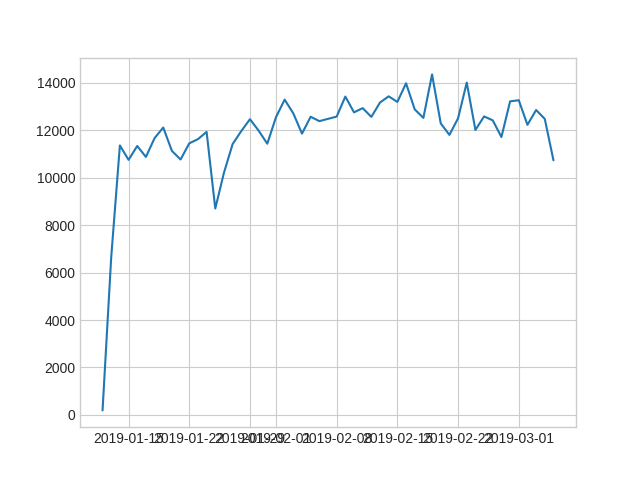
\includegraphics[width=0.85 \textwidth]{src/images/over_time.png}
        \caption{Rate of attacks from 12. Jan to 5. March}
        \label{fig:attacks_over_time}
    \end{figure}


    If the same done over the week (see figure \ref{fig:over_week}), 
    there is a seemingly
    non-random pattern that can be discerned, in that 
    over the weekend, the rate becomes more varied.


    \begin{figure}[H]
        \centering
        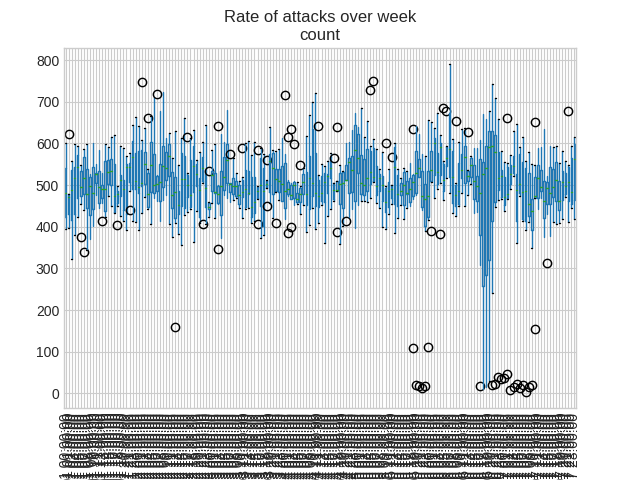
\includegraphics[width=0.8\textwidth]{src/images/week_unfiltered.png} 
        \caption{Rate of attacks plotted over a 'typical' week.}
        \label{fig:over_week}
    \end{figure}

    To preform the next two tests, I grouped the attacks by the
    date and time that they were launched, then grouped them 
    again by the time of day they were launched, taking the
    mean of the attack rates.

    To discover if there exists a relationship between the 
    time of day and attacks received, I attempted to use 
    autocorrelation as provided by the pandas library,
    but did not yield significant results. Either meaning that
    there is no correlation, or that the correlation is not 
    linear. 

    To discover if the mean attack rates over each hour of the
    day are likely to have been observations drawn from the same
    distributions, I preformed an 
    analysis of variance test (\textit{ANOVA}). 
    For this test I included all weekdays.

    This test resulted in a P value of 0.0395, which
    is enough to reject the hypothesis that the distributions
    of attacks over the hours of the day are equivalent (see table
    \ref{tab:anova_launches}).


    % df       sum_sq     mean_sq         F    PR(>F)
    % count       1.0   169.713862  169.713862  3.575061  0.060396
    % Residual  166.0  7880.286138   47.471603       NaN       NaN
    \begin{table}[H]
        \centering
        \begin{tabular}{|l|l|l|l|l|l|}
            \hline
                 & df    & sum\_sq     & mean\_sq   & F        & PR(\textgreater{}F) \\ \hline
        count    & 1.0   & 169.713862  & 169.713862 & 3.575061 & 0.060396            \\ \hline
        Residual & 166.0 & 7880.286138 & 47.471603  & NaN      & NaN \\\hline  
        \end{tabular}
        \caption{Anova Results for attack launch rate and time of day}
        \label{tab:anova_launches}
    \end{table}

    Graphing the rate of attacks launched suggests that 
    it is most popular for hackers to launch their attacks at
    around 05:00 in the morning (see figure \ref{fig:over_day})

    \begin{figure}[H]
        \centering
        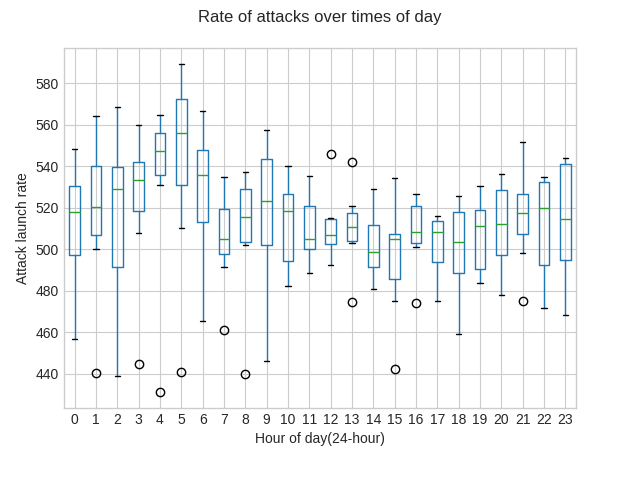
\includegraphics[width=0.85\textwidth]{src/images/rate_over_day.png}
        \caption{Anova results on testing rates of attacks launched over the time of day.}
        \label{fig:over_day}
    \end{figure}

    Repeating this test for the rates of attacks received, 
    does not yield a P value significant at the 0.05 level (see 
    table \ref{tab:anova_received}),
    however graphing it still shows the 05:00 peak. 
    
    \begin{table}[H]

        \centering
        \begin{tabular}{|l|l|l|l|l|l|}
        \hline
                 & df    & sum\_sq     & mean\_sq   & F        & PR(\textgreater{}F) \\ \hline
        count    & 1.0   & 169.713862  & 169.713862 & 3.575061 & 0.060396            \\ \hline
        Residual & 166.0 & 7880.286138 & 47.471603  & NaN      & NaN                 \\ \hline
        \end{tabular}
        \caption{Anova results on testing rates of attacks received over the time of day.}
        \label{tab:anova_received}
    \end{table}


    \begin{figure}[H]
        \centering
        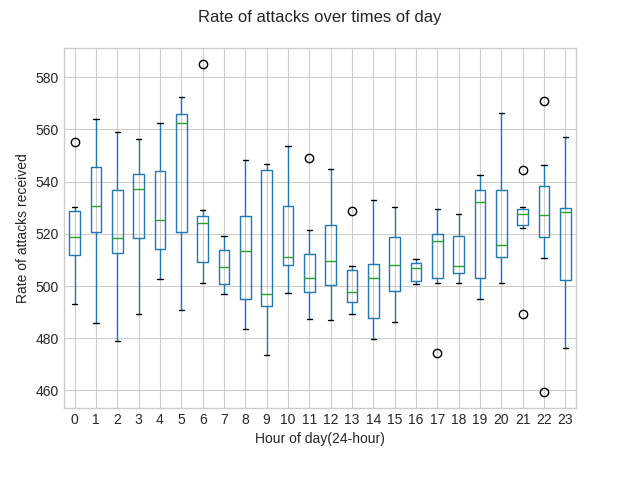
\includegraphics[width=0.85\textwidth]{src/images/rate_over_day_received.png}
        \caption{Rates of attacks received over the time of day.}
        \label{fig:over_day}
    \end{figure}

\subsection{Session log analysis}
\label{sec:session_analysis}

    The cowrie honeypot also captures the actions of 
    the attacker, as well as the files which he attempts
    to download and run on what he thinks is a compromised
    server. 


    One of the more intriguing factors that a number of the
    attack logs show, is an attempt to access a command
    called \texttt{'\\gisdfoewrsfdf'}. A command that 
    has I do not know what does, and a search yields no
    definitive results to what this command or script is. 

    Amongst the other things that are attempted, 
    are wiping the \texttt{./ssh/authorized\_keys} file and
    inserting a key, presumably of another infected
    device. 

    Twice during the period of 12. January to 1. March, 
    an attacker tried to download, and start an IRC bot.

    

\subsection{Origin of attacks}
\label{sec:origin_analysis}


    The most common countries of origin are Ireland, Russia,
    Germany, the Netherlands, and China.

    \begin{figure}[H]
        \centering
        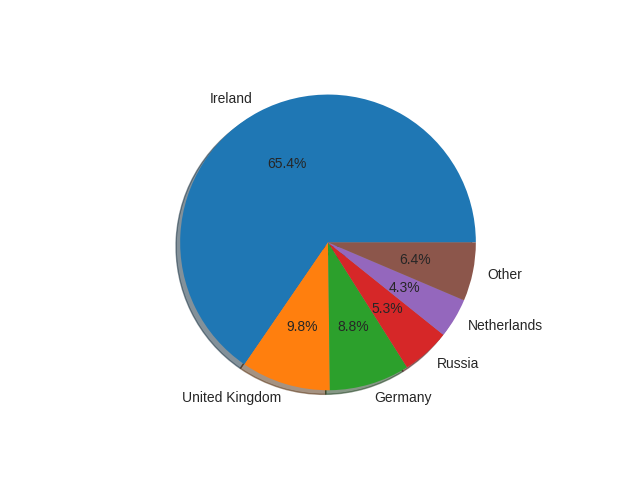
\includegraphics[width=0.8\textwidth]{src/images/countries_pie.png}
        \caption{Most common countries of origin.}
        \label{fig:country_pie}
    \end{figure}

    It was surprising how large the amount of attacks came from
    Ireland, and in fact upon closer inspection, 
    \texttt{'5.188.86.174'} is the originator of 
    $7.7\%$ of all attacks 
    (see figure \ref{fig:attacks_by_ip}).

    \begin{figure}[H]
        \centering
        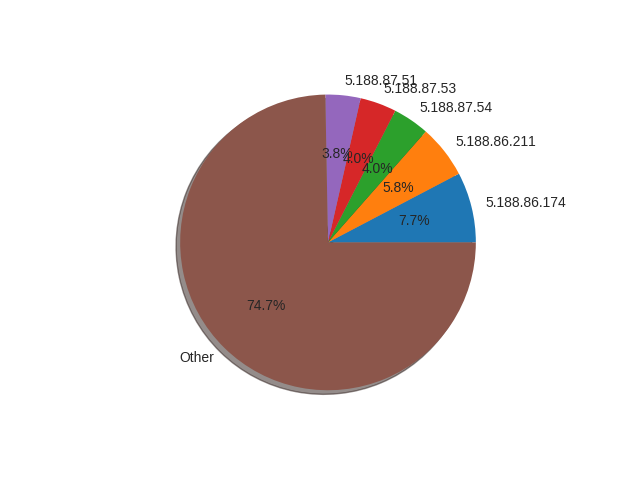
\includegraphics[width=0.8\textwidth]{src/images/ip_breakdown.png}
        \caption{Total attacks broken down by source address}
        \label{fig:attacks_by_ip}
    \end{figure}


    In fact, looking into the top offenders, 


    \texttt{'5.188.86.174'},
    \texttt{'5.188.86.211'},
    \texttt{'5.188.87.53'},
    \texttt{'5.188.87.54'}, and 
    \texttt{'5.188.87.55'} 

    reveals that all of them 
    are owned by \texttt{'Petersburg 
    Internet Network ltd.'}\abbrv{PIN}, a russian service provider 
    which has been implicated in both route-hijacking \cite{bogus_routing} 
    and allegedly with a gang of cyber criminals \cite{petersburg}

    
    A quick scan of the top offender, \texttt{'5.188.86.174'},
    preformed on the 19. of March revealed that it was a part of
    a TOR network. A secondary scan on the 4. of 
    April showed that the TOR ports were closed.

    This does not necessarily mean that all traffic from PIN
    registered IPs are russian in origin, but should be 
    subject for further inspection.
\section{Discussion}
\label{sec:discussion}
% \section{Results}
\label{sec:results}

    The honeypot records both time stamps, and 
    interaction logs. Analysis of each will be handled separately 
    in subsections \ref{sec:time_analysis} and 
    \ref{sec:session_analysis}. 

    Then in section \ref{sec:irish_analysis} I take 
    a brief look at the origins of attacks.

\subsection{Statistical analysis of attack data}
\label{sec:time_analysis}

    The honeypot has been active since 12. of January
    2019, and until the 19. of March has logged 
    812013 individual SSH attacks. 


    The rate of attacks has been relatively constant over
    time (see figure \ref{fig:attacks_over_time}), with 
    the notable exception of the 12. of January and of 25. 
    January. The low amount of attacks on 12. of January is due 
    to how late I set the server up. 
    The dip in attack rate on the 25 is as of yet 
    unexplained.


    \begin{figure}[H]
        \centering
        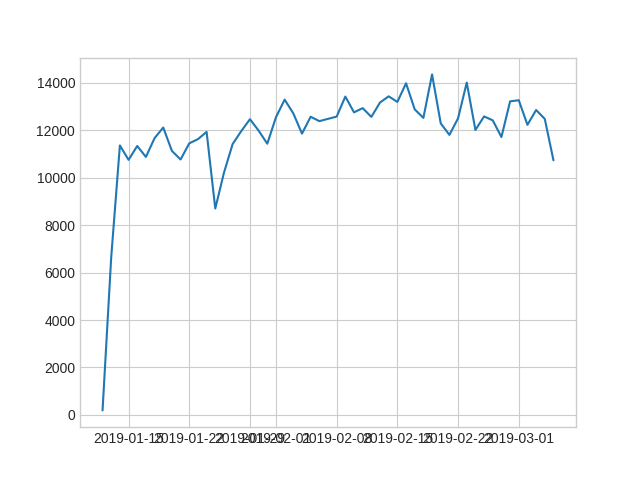
\includegraphics[width=0.85 \textwidth]{src/images/over_time.png}
        \caption{Rate of attacks from 12. Jan to 5. March}
        \label{fig:attacks_over_time}
    \end{figure}


    If the same done over the week (see figure \ref{fig:over_week}), 
    there is a seemingly
    non-random pattern that can be discerned, in that 
    over the weekend, the rate becomes more varied.


    \begin{figure}[H]
        \centering
        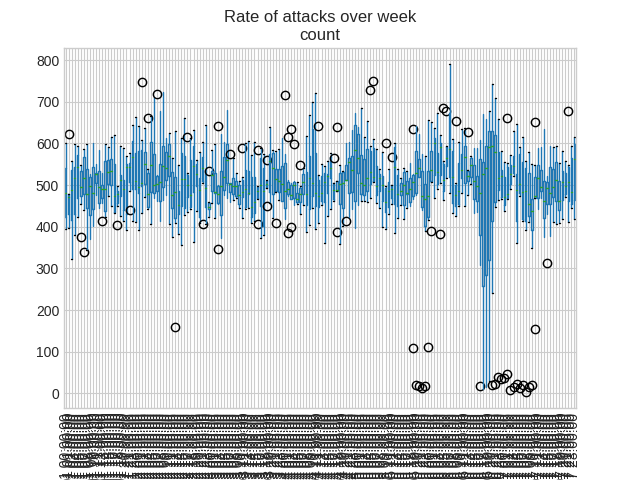
\includegraphics[width=0.8\textwidth]{src/images/week_unfiltered.png} 
        \caption{Rate of attacks plotted over a 'typical' week.}
        \label{fig:over_week}
    \end{figure}

    To preform the next two tests, I grouped the attacks by the
    date and time that they were launched, then grouped them 
    again by the time of day they were launched, taking the
    mean of the attack rates.

    To discover if there exists a relationship between the 
    time of day and attacks received, I attempted to use 
    autocorrelation as provided by the pandas library,
    but did not yield significant results. Either meaning that
    there is no correlation, or that the correlation is not 
    linear. 

    To discover if the mean attack rates over each hour of the
    day are likely to have been observations drawn from the same
    distributions, I preformed an 
    analysis of variance test (\textit{ANOVA}). 
    For this test I included all weekdays.

    This test resulted in a P value of 0.0395, which
    is enough to reject the hypothesis that the distributions
    of attacks over the hours of the day are equivalent (see table
    \ref{tab:anova_launches}).


    % df       sum_sq     mean_sq         F    PR(>F)
    % count       1.0   169.713862  169.713862  3.575061  0.060396
    % Residual  166.0  7880.286138   47.471603       NaN       NaN
    \begin{table}[H]
        \centering
        \begin{tabular}{|l|l|l|l|l|l|}
            \hline
                 & df    & sum\_sq     & mean\_sq   & F        & PR(\textgreater{}F) \\ \hline
        count    & 1.0   & 169.713862  & 169.713862 & 3.575061 & 0.060396            \\ \hline
        Residual & 166.0 & 7880.286138 & 47.471603  & NaN      & NaN \\\hline  
        \end{tabular}
        \caption{Anova Results for attack launch rate and time of day}
        \label{tab:anova_launches}
    \end{table}

    Graphing the rate of attacks launched suggests that 
    it is most popular for hackers to launch their attacks at
    around 05:00 in the morning (see figure \ref{fig:over_day})

    \begin{figure}[H]
        \centering
        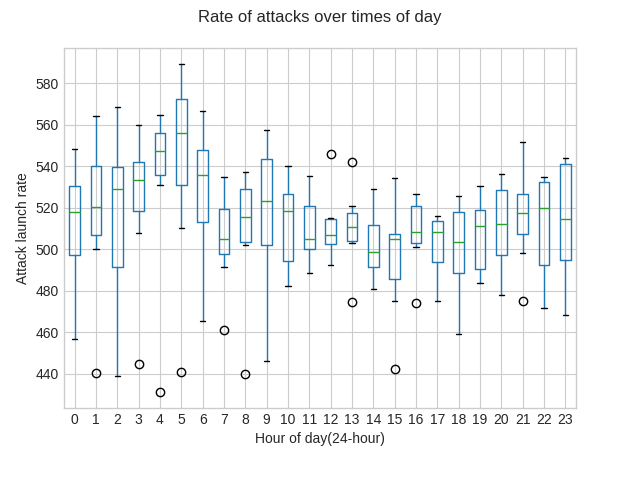
\includegraphics[width=0.85\textwidth]{src/images/rate_over_day.png}
        \caption{Anova results on testing rates of attacks launched over the time of day.}
        \label{fig:over_day}
    \end{figure}

    Repeating this test for the rates of attacks received, 
    does not yield a P value significant at the 0.05 level (see 
    table \ref{tab:anova_received}),
    however graphing it still shows the 05:00 peak. 
    
    \begin{table}[H]

        \centering
        \begin{tabular}{|l|l|l|l|l|l|}
        \hline
                 & df    & sum\_sq     & mean\_sq   & F        & PR(\textgreater{}F) \\ \hline
        count    & 1.0   & 169.713862  & 169.713862 & 3.575061 & 0.060396            \\ \hline
        Residual & 166.0 & 7880.286138 & 47.471603  & NaN      & NaN                 \\ \hline
        \end{tabular}
        \caption{Anova results on testing rates of attacks received over the time of day.}
        \label{tab:anova_received}
    \end{table}


    \begin{figure}[H]
        \centering
        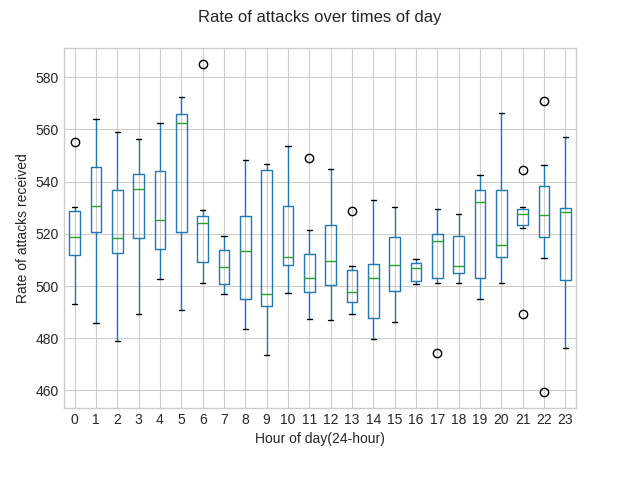
\includegraphics[width=0.85\textwidth]{src/images/rate_over_day_received.png}
        \caption{Rates of attacks received over the time of day.}
        \label{fig:over_day}
    \end{figure}

\subsection{Session log analysis}
\label{sec:session_analysis}

    The cowrie honeypot also captures the actions of 
    the attacker, as well as the files which he attempts
    to download and run on what he thinks is a compromised
    server. 


    One of the more intriguing factors that a number of the
    attack logs show, is an attempt to access a command
    called \texttt{'\\gisdfoewrsfdf'}. A command that 
    has I do not know what does, and a search yields no
    definitive results to what this command or script is. 

    Amongst the other things that are attempted, 
    are wiping the \texttt{./ssh/authorized\_keys} file and
    inserting a key, presumably of another infected
    device. 

    Twice during the period of 12. January to 1. March, 
    an attacker tried to download, and start an IRC bot.

    

\subsection{Origin of attacks}
\label{sec:origin_analysis}


    The most common countries of origin are Ireland, Russia,
    Germany, the Netherlands, and China.

    \begin{figure}[H]
        \centering
        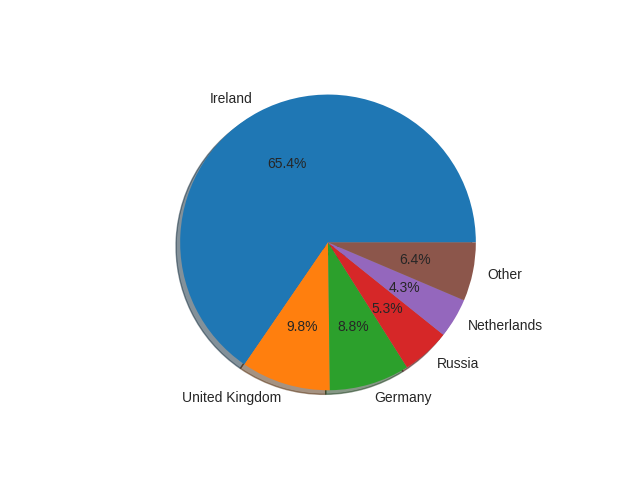
\includegraphics[width=0.8\textwidth]{src/images/countries_pie.png}
        \caption{Most common countries of origin.}
        \label{fig:country_pie}
    \end{figure}

    It was surprising how large the amount of attacks came from
    Ireland, and in fact upon closer inspection, 
    \texttt{'5.188.86.174'} is the originator of 
    $7.7\%$ of all attacks 
    (see figure \ref{fig:attacks_by_ip}).

    \begin{figure}[H]
        \centering
        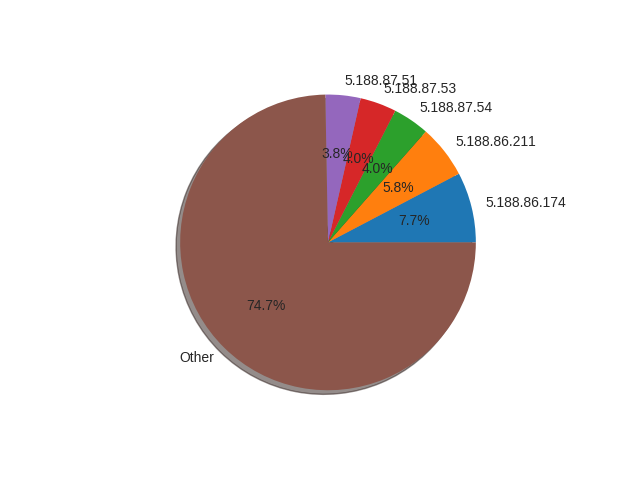
\includegraphics[width=0.8\textwidth]{src/images/ip_breakdown.png}
        \caption{Total attacks broken down by source address}
        \label{fig:attacks_by_ip}
    \end{figure}


    In fact, looking into the top offenders, 


    \texttt{'5.188.86.174'},
    \texttt{'5.188.86.211'},
    \texttt{'5.188.87.53'},
    \texttt{'5.188.87.54'}, and 
    \texttt{'5.188.87.55'} 

    reveals that all of them 
    are owned by \texttt{'Petersburg 
    Internet Network ltd.'}\abbrv{PIN}, a russian service provider 
    which has been implicated in both route-hijacking \cite{bogus_routing} 
    and allegedly with a gang of cyber criminals \cite{petersburg}

    
    A quick scan of the top offender, \texttt{'5.188.86.174'},
    preformed on the 19. of March revealed that it was a part of
    a TOR network. A secondary scan on the 4. of 
    April showed that the TOR ports were closed.

    This does not necessarily mean that all traffic from PIN
    registered IPs are russian in origin, but should be 
    subject for further inspection.
\section{Conclusion}
\label{sec:conclusion}

In this paper I have described the process of setting up a HonePot
server with Modern Honey Network. I have also described how I 
processed the data, and how I preformed the statistical analysis.


I found that both the rate of attacks received and the rate 
of attacks launched did not have a strong linear correlation
to the time of day. 


An ANOVA test preformed on the rate of attacks received over 
the time of day showed that there is a difference in rates
significant at the 0.06 level.


If the same test is preformed on the
 time which the attacks
were launched, the difference is now significant at the 0.03
level.


There seems to be a peak of attacks launched at 
05:00 (see figure \ref{fig:over_day}), this may be 
because attackers assume that the security staff is 
not as responsive at such a late hour. But seeing as
how 90\% of attacks come from foreign time zones, this 
seems unlikely to be the reason.


Future work could be repeating this experiment in different
countries, collecting data over longer periods, figuring out
given a pattern, if it can be localized to a timezone.


% \noindent Displayed equations are centered and set on a separate
% line.
% \begin{equation}
% x + y = z
% \end{equation}
% Please try to avoid rasterized images for line-art diagrams and
% schemas. Whenever possible, use vector graphics instead (see
% Fig.~\ref{fig1}).


% \begin{theorem}
% This is a sample theorem. The run-in heading is set in bold, while
% the following text appears in italics. Definitions, lemmas,
% propositions, and corollaries are styled the same way
% \end{theorem}
% 
% the environments 'definition', 'lemma', 'proposition', 'corollary',
% 'remark', and 'example' are defined in the LLNCS documentclass as well.
%
% \begin{proof}
% Proofs, examples, and remarks have the initial word in italics,
% while the following text appears in normal font.
% \end{proof}
    % \printbibliography
    \clearpage
    \bibliographystyle{ieeetr}
    \bibliography{src/Citations}
    % \bibliographystyle{plain}

\end{document}
